\documentclass[10pt, conference]{IEEEtran}



\usepackage{cmap}  \usepackage[T1]{fontenc}  \usepackage[utf8]{inputenc}
\usepackage{microtype}  


\usepackage{amsmath,amssymb,graphicx}
\usepackage{txfonts}
\usepackage{stmaryrd}
\usepackage{url}
\usepackage[english]{babel}

\usepackage{hyperref}


\usepackage{tikz}

\DeclareMathOperator{\Ai}{Ai}
\DeclareMathOperator{\erf}{erf}
\DeclareMathOperator{\EXP}{Exp}
\newcommand{\abs}[1]{\mathopen|#1\mathclose|}
\newcommand{\ttarget}{p}
\newcommand{\twork}{t}
\newcommand{\R}{\mathbb{R}}
\newcommand{\Z}{\mathbb{Z}}
\newcommand{\rnd}[1]{\left\langle #1 \right\rangle}
\newcommand{\transp}[1]{#1^{\operatorname T}}

\renewcommand{\Phi}{\mathcal{F}}
\usepackage[english, ruled, vlined, linesnumbered]{algorithm2e}
\SetAlCapSkip{\abovecaptionskip}
\SetKwComment{tc}{}{}
\SetKwRepeat{doWhile}{do}{while}
\SetKwFunction{KwImplementer}{implementer}
\SetKwFunction{KwOutput}{output}
\SetKwData{Nv}{N}
\SetKwData{Mv}{M}
\SetKwData{yv}{y}
\SetKwData{av}{a}
\SetKwData{bv}{b}
\SetKwData{tmpv}{tmp}

\newtheorem{corollary}{Corollary}
\newtheorem{lemma}{Lemma}
\newtheorem{notation}{Notation}
\newtheorem{remark}{Remark}
\newtheorem{proposition}{Proposition}
\newtheorem{theorem}{Theorem}

\newcommand{\assign}{:=}
\newcommand{\emdash}{---}
\newcommand{\mathd}{\mathrm{d}}
\newcommand{\nocomma}{}
\newcommand{\nosymbol}{}
\newcommand{\tmop}[1]{\ensuremath{\operatorname{#1}}}
\newcommand{\tmtextit}[1]{{\itshape{#1}}}



\begin{document}

\setlength{\emergencystretch}{1em}
\abovedisplayskip=3pt plus 4pt
\abovedisplayshortskip=0pt plus 3pt
\belowdisplayskip=3pt plus 4pt
\belowdisplayshortskip=0pt plus 3pt
\setlength{\textfloatsep}{5pt} 
\setlength{\abovecaptionskip}{0pt}
\setlength{\belowcaptionskip}{0pt}

\title{Multiple-precision evaluation of the Airy  function with
reduced cancellation}
\author{
    \IEEEauthorblockN{Sylvain Chevillard\\}
    \IEEEauthorblockA{
        Inria, Apics Project-Team, Sophia Antipolis, France\\
\href{mailto:sylvain.chevillard@inria.fr}{sylvain.chevillard@inria.fr}
    }
    \and
    \IEEEauthorblockN{Marc Mezzarobba\\}
    \IEEEauthorblockA{
        Inria, LIP (CNRS-ENS-Inria-UCBL), ENS de  Lyon, France\\
\href{mailto:marc@mezzarobba.net}{marc@mezzarobba.net}
    }
}
\maketitle


\begin{abstract}
The series expansion at the origin of the Airy function~ is alternating and hence problematic to evaluate for  due to cancellation.
Based on a method recently proposed by Gawronski,
M\"uller, and Reinhard, we exhibit two functions ~and~, both with
nonnegative Taylor expansions at the origin, such that . The sums are now well-conditioned, but the Taylor coefficients
of~ turn out to obey an ill-conditioned three-term recurrence. We use the
classical Miller algorithm to overcome this issue. We bound
all errors and our implementation allows an arbitrary and certified accuracy,
that can be used, e.g., for providing correct rounding in arbitrary precision.
\end{abstract}

\begin{IEEEkeywords}
Special functions; algorithm; numerical evaluation; arbitrary precision; Miller method; asymptotics; correct rounding; error bounds.
\end{IEEEkeywords}

\newcommand\mightbeomitted{}



Many mathematical functions (e.g., trigonometric functions, , Bessel functions) have a Taylor series of the form

with  and .
For large , the computation in finite precision arithmetic of such a sum
is notoriously prone to {\emph{catastrophic cancellation}}.
Indeed, the terms  are first growing before the series ``starts to
converge'' when . In particular, when ,
the terms  usually get much larger than~. Eventually, their leading
bits cancel out while lower-order bits that actually contribute to the first
significant digits of the result get lost in roundoff errors.

This cancellation phenomenon makes the direct
computation by Taylor series impractical for large values of .
Often, the function~ admits an asymptotic expansion as
{}
that can be used very effectively to obtain numerical approximations when~
is large, but might not provide enough accuracy (at least without resorting to sophisticated resummation methods) for intermediate values of~.

In the case of the error function , a
classical trick going back at least to Stegun and
Zucker~{\cite{StegunZucker1970}} is to compute 
as  where  and~{\cite[Eq.~7.6.2]{DLMF}}

The benefit of this transformation is that ~and~ are power series with
nonnegative coefficients, and can thus be computed without cancellation.
Algorithms based on~\eqref{eq:std recond erf} tend to behave well in some
range  where ~is large enough for cancellation to be problematic
but small enough to make the use of asymptotic expansions at infinity
inconvenient.
Note that the obvious way to compute  for  fits into the same framework, now with 
and .

Gawronski, M\"uller and
Reinhard~{\cite{GawronskiMullerReinhard2007,Reinhard2008}} provide elements to
understand where these rewritings ``come from''. They relate the amount of
cancellation in the summation of a series~\eqref{eq:intro} to the shape of the
Phragm\'en--Lindel\"of indicator of~, a classical tool from the theory of
entire functions~{\cite{Levin1996}}. This description allows them to state
criteria for choosing auxiliary series suitable for the evaluation of a given
entire function in a given sector of the complex plane. They apply their
method (called the ``GMR method'' in what follows) to obtain ``reduced
cancellation'' evaluation algorithms for the error function and other related
functions in various sectors.

In this article, we are interested in the evaluation for positive~ of the
Airy function ~\cite[Chap.~9]{DLMF}.
The function  satisfies the linear ordinary
differential equation (LODE)

with initial values

The classical existence theorem for LODE with complex analytic coefficients
implies that  is an entire function; and
solving~\eqref{eq:deq Ai} by the method of power series yields the Taylor
expansion , where

Observe that while ~and~ are easy enough to evaluate individually, the
difference~ causes catastrophic cancellation when computed in
approximate arithmetic.

Using the GMR method, we derive a reduced cancellation algorithm for
computing .
To our best knowledge, our algorithm for evaluating  is new, and is the
most efficient multiple-precision evaluation of 
when  is neither too small nor too large, while the precision is not large
enough to make methods based on binary splitting~\cite{BrentZimmermann2010} competitive.

Besides the new application, the main difference between the
present article and the work of Gawronski {\emph{et al.}} is our setting of
multiple-precision arithmetic ``\`a la
MPFR~{\cite{FousseHanrotLefevrePelissierZimmermann2007}}''. Specifically, on
the one hand, we are interested in {\emph{arbitrary precision}} arithmetic
rather than machine precision only. This makes it impossible, for instance, to
tabulate the coefficients of auxiliary functions when these turn out to be
hard to compute. Also, we are looking for {\emph{rigorous error bounds}}
instead of experimental error estimates. On the other hand, we restrict
ourselves to numerical evaluation on a half line instead of a complex sector (though, in principle, the basic ideas generalize).

This article focuses on providing a complete algorithm in the specific
case of , . Yet, it should also be seen a
{\emph{case study}}, part of an effort to understand what the GMR method can
bring in the context of multiple-precision computation, and, perhaps more
importantly, how general and systematic it can be made. We discuss this last
point further in Sec.~\ref{sec:conclusion}.

The rest of this text is organized as follows.
In Sec.~\ref{sec:GMR}, we use the GMR method to choose the functions ~and~.
Then, in Sec. \ref{sec:F}~and~\ref{sec:G}, we derive a few mathematical properties of these functions, including recurrences for their series expansions and various bounds.
Sections~\ref{sec:roundoff Analysis} to~\ref{sec:evaluation of F} contain the details of our algorithm and its error analysis.
Finally, in Sec.~\ref{sec:implementation}, we briefly describe our implementation of the algorithm.

\section{The GMR method}
\label{sec:GMR}

We now review the GMR method and apply it to obtain candidate
auxiliary series for the evaluation of the  function. Since the
method itself is not crucial for our results, we summarize it in intuitive
terms and refer the reader to the original
works~{\cite{GawronskiMullerReinhard2007,Reinhard2008}} for more careful
statements.

\newcommand\myfrac[2]{#1/#2}
\newcommand\axes{
  \draw[->] (0,-2/3-0.1) -- (0,4/3+0.2);
  \draw[->] (-pi-.2,0) -- (pi+.2,0);
  \begin{scope}[inner sep=1pt, outer sep=2pt]
    \foreach \x / \xtext in {
          -pi / -\pi,
          -0.666*pi / -\myfrac{2\pi}{3},
          -0.333*pi / -\myfrac\pi3,
          0.333*pi / \myfrac\pi3,
          0.666*pi / \myfrac{2\pi}{3},
          pi / \pi,
    }
      \draw (\x,1pt) -- (\x,-1pt) node[below, fill=white] {};
    \foreach \i in {-2, 2, 4}
      \draw (1pt,\i/3) -- (-1pt,\i/3) node[left, fill=white] {};
    \end{scope}
}
\tikzset{x=.64cm,y=.8cm,font=\scriptsize}

\begin{figure}
\centerline{
    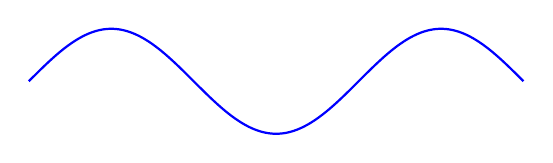
\begin{tikzpicture}
      \draw[color=blue,thick] plot[smooth,domain=-pi:pi,samples=100]
        (\x, {-2/3*cos(1.5*\x r)});
      \axes
    \end{tikzpicture}
  }
  \caption{The indicator function  of .\label{fig:h Ai}}
\end{figure}

The starting point of the GMR method is the following observation. Let  be an entire function. Assume
that we have, in some intentionally vague sense,

for large~. (To make things precise, we would assume that  has finite
{\emph{order}} , and that ~is its {\emph{indicator function}} with
respect to~~{\cite{Levin1996}}.)

We consider the computation of~ in floating-point
arithmetic using its series expansion. It is well-known~\cite{Chevillard2012} that, if the sum is performed in floating-point arithmetic of precision~, the relative error between  and the computed sum is roughly given by . The sum  is larger than , and usually of the same order of magnitude. Therefore, the number of significant binary digits ``lost by cancellation'' is roughly


Denote

for all .
Cauchy's formula implies , and under a suitable version of
hypothesis~\eqref{eq:or mag y}, one can actually show that . Hence, the loss of
precision by cancellation in the evaluation of  is about

For instance, when the  all have the same complex argument, the maximum
of~ is reached for~, in accordance with the fact that the sum
is optimally conditioned.

In the case of the Airy  function, the following asymptotic
equivalent holds as ~tends to complex infinity in any open sector that
avoids the negative real axis~{\cite[Eq.~9.7.5]{DLMF}}:

Additionally,  is bounded for . Hence, we
may take  and

(see Figure~\ref{fig:h Ai}). The loss of precision is roughly proportional to
. It is minimal in the directions of fastest
growth , and maximal for~.

If now two entire functions ~and~ both satisfy conditions of the
form~\eqref{eq:or mag y} with the same~ but different~ (say  and
, respectively), we may expect that

The GMR method consists in reducing the summation of the series~ for  in
some given sector to that of an {\emph{auxiliary series}} 
and a {\emph{modified series}}  related by~\eqref{eq:hG}.
The value of  is then recovered as . The auxiliary series is chosen, based on the shape
of~, so that both  and  take values close to their
maximum in the sector of interest.



There may be multiple choices, and it is not clear in general which one is better, except that the coefficients of ~and~ should be as easy to compute as possible.
Gawronski {\emph{et al.}} usually take  and search for a value of~ that makes  as small as possible on a whole complex sector. The choice of
exponentials as auxiliary series is not appropriate in the case of
, since  is an entire function of~
only for integer~.


However, as we are interested in one direction only, we can easily build a
suitable auxiliary series from~ itself. Indeed, we may ``shift''
the indicator function of~ by  to the left or to the
right by changing  to , where . (Note
that this is {\emph{not}} the same as changing~ to  in~\eqref{eq:h Ai}.) When we add such a shifted
indicator to the original~, one of the humps of the curve cancels out with
the valley in the middle.

\begin{figure}
\begin{tikzpicture}
    \draw[blue,thick] plot[smooth,domain=-pi/3:pi/3] (\x, {4/3*cos(1.5*\x r)});
    \axes
    \begin{scope}[color=blue, thick]
      \draw (-pi,0) -- (-pi/3,0);
      \draw (pi/3,0) -- (pi,0);
    \end{scope}
  \end{tikzpicture}
  \hfill
  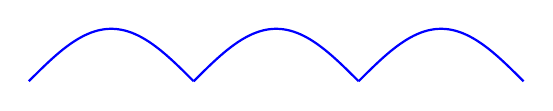
\begin{tikzpicture}
    \begin{scope}[color=blue, thick]
      \draw plot[smooth,domain=-pi/3:pi/3] (\x, {2/3*cos(1.5*\x r)});
      \draw plot[smooth,domain=-pi/3:pi/3] (\x-2/3*pi, {2/3*cos(1.5*\x r)});
      \draw plot[smooth,domain=-pi/3:pi/3] (\x+2/3*pi, {2/3*cos(1.5*\x r)});
    \end{scope}
    \axes
  \end{tikzpicture}
  \caption{Indicator functions for~ (left) and~ (right).\label{fig:h F G}}
\end{figure}

Using this idea, we set

The indicator functions of ~and~ are pictured on Figure~\ref{fig:h F G}.
Based on their shapes, we expect that both series are optimally conditioned on
the positive real axis.
We shall prove that this is indeed the case in the
next two sections.

This second method of constructing auxiliary series seems to be new, and applies to many cases.
For instance, applying it to the error function leads to


a slightly worse alternative to~\eqref{eq:std recond erf}.
The advantage of~\eqref{eq:std recond erf} comes from the fact that  is faster to evaluate than~\eqref{eq:new recond erf}.


\section{The auxiliary series~}
\label{sec:F}

The functions ~and~ being chosen, we need to establish appropriate formulas to evaluate them, along with error bounds.
Much of our analysis will be based on the following simple
estimate~{\cite[Chap.~4, {\S}4.1]{Olver1997}}, where  was defined in Eq.~\eqref{eq:Ai-tilde}.

\begin{lemma}
  \label{lem:asympt approx Ai}The Airy function~ satisfies
  
  where
  .
\end{lemma}

Now consider the power series expansion of~ at the origin:


\begin{proposition}
  \label{prop:rec F}The coefficients~ are positive and satisfy the
  two-term recurrence relation
  
  with initial values
  
  
\end{proposition}

\begin{IEEEproof}
  As a general fact, if two functions ~and~ each satisfy a
  homogeneous LODE with coefficients in~, then
  their product  satisfies an equation of the same class that can be explicitly computed~{\cite[Sec.~6.4]{Stanley1999}}.
The functions  satisfy the same
  differential equation~\eqref{eq:deq Ai} as~
  itself. Applying the procedure mentioned above
  to two copies of that equation yields .
  
  Similarly, when an analytic function~ satisfies a homogeneous LODE
  over~, we can compute a recurrence relation with
  coefficients in~ on the coefficients~ of its power
  series expansion.
  In the case of~, we get~\eqref{eq:rec F}. Finally, we
  compute the initial values  from the first few terms of the
  Taylor expansion of :
  
  It is then apparent from~\eqref{eq:rec F} that  for all .
\end{IEEEproof}

Thus, the coefficients of  obey a two-term recurrence
whose coefficients do not vanish for . This allows one to
compute them in a numerically stable way (see Sec.~\ref{sec:evaluation of F}).




\section{The modified series }
\label{sec:G}

Recall that , and set


\begin{proposition}
  \label{prop:rec G}
  The function  is an entire function with power series
  expansion of the form .
  The coefficient sequence  is
  determined from its first terms
  
  by the recurrence relation
  
\end{proposition}

\begin{IEEEproof}
  First, observe that  and , so that the Taylor
  expansion of~ at the origin is a power series in~ with
  real coefficients. The same routine reasoning as in the proof of
  Prop.~\ref{prop:rec F} yields the LODE
  
  and from there the recurrence~\eqref{eq:rec G}. The coefficients
  of~\eqref{eq:rec G} do not vanish for , so that the
  sequence~ is indeed determined by , , and \eqref{eq:rec G}.
\end{IEEEproof}

Nonzero solutions of~\eqref{eq:rec G} decrease roughly as  for
large~.
Setting~ yields the
``normalized'' recurrence

Letting ~go to infinity in the coefficients of~\eqref{eq:norm rec G}, we
get a limit recurrence with constant coefficients whose
characteristic polynomial  has two roots of
distinct absolute value, namely ~and~. By the Perron--Kreuser
theorem~{\cite[Theorem~B.10]{Wimp1984}}, it follows that any solution~ of~\eqref{eq:rec G} satisfies

with either  or . Solutions  such that  are called
{\emph{minimal}} and form a linear subspace of dimension~ of the solutions of~\eqref{eq:rec G}.

We shall prove that~ actually is such a minimal solution of~(\ref{eq:rec
G}). But our analysis uses a bit more than the rough estimate . Prop.~\ref{prop:bound on Gn} below
provides a more precise estimate which implies the minimality.
Before turning to it, we recall a standard bound on the tails of incomplete Gaussian integrals~{\cite[Eq.~7.12.1]{DLMF}} and state a second technical lemma.

\begin{lemma}
  \label{lem:erf}The complementary error function
  
  satisfies
  
  for .
\end{lemma}

\begin{lemma} \label{lem:int} \mightbeomitted
  \label{lem:I2-I1}The expression
  
  satisfies  for all .
\end{lemma}

\begin{IEEEproof}
  We first use the inequality  (valid for )
  followed by the change of variable  to get
  
  where  and . Now we have
  
  and, by Lemma~\ref{lem:erf},
  .
  When , the last bound is decreasing and hence less than~.
\end{IEEEproof}

The following proposition is the main result of this section and the starting point of much of the error analysis that follows.
Though somewhat technical, the proof is mostly routine.

\begin{proposition}
  \label{prop:bound on Gn}The sequence~ satisfies
  
  with relative error
   \hspace{1em}().
\end{proposition}

\begin{notation} \label{not:E}
  We write
  ,
  so that, if  for all , then  with .
  Note that we obviously have  for .
\end{notation}

\begin{IEEEproof}
  The proof is a standard application of the {\emph{saddle point method}}
\cite[{\S}VIII.3]{FlajoletSedgewick2009}, which we work out in
  some detail in order to get an explicit error bound.

  We fix . We shall write  in the following.
  The method prescribes to choose , so that
  
  (i.e., ).

  Now, guided by~\eqref{eq:saddle cond} and , we write
  
  Most of the weight of  is concentrated around . We set
  
  Since , we remark that  and .
  We further let
  

  We first bound the error between  and . When ,
  using Lemma~1 and the connection formula~{\cite[Eq. 9.2.12]{DLMF}}
  
  we see that {} is
  bounded by
  
  It follows that  when .
  By symmetry, this inequality holds for  too.
Finally, we have
  
  and hence, using Lemma~\ref{lem:I2-I1},
  

  We now have to estimate . We write
  
  On the one hand, Lemma~\ref{lem:asympt approx Ai} gives
   with
   where .
  Note that this bound increases with~.

  On the other hand, thanks to~\eqref{eq:saddle cond}, we can write
  
  where
  
  Let
  
  Since  by the
  choice~\eqref{eq:theta0}, using~\eqref{eq:bound u} and the
  inequality , we
  have, for  and :
  
  To sum up, we can now rewrite  as
  

  Now, define
  
  When , we have
  
  so we get
  
  Finally,  is an incomplete Gaussian integral:
  
  Lemma~\ref{lem:erf} yields
  
  Putting together (\ref{eq:bound B}, \ref{eq:bound C},
  \ref{eq:bound D}), we obtain  with
  

  Now, we can write  with
  
  Stirling's formula in the form~\cite{Robbins1955}
  ,
  combined with the bound
  ,
  yields
  
  It follows that
  
  One easily checks that this bound is valid for
  .
\end{IEEEproof}

Note that the above bound is not the best we can get by this method.
Indeed, by choosing the exponent of~ in~\eqref{eq:theta0} closer to , we obtain~ for any . This comes at the price of a larger constant factor and thus more terms to check separately.

A first consequence of Prop.~\ref{prop:bound on Gn} is that the series~ has nonnegative coefficients, as stated below.
We also deduce several other technical results that will be used to bound various error terms.
Recall that , and let .

\begin{corollary}
    \label{cor:positivity}  The sequence  satisfies  for all . Accordingly, we have .
    In particular, the~ are positive.
\end{corollary}

\begin{IEEEproof}
 Prop.~\ref{prop:bound on Gn} implies that  with . When , we have . This implies  and
  .
  The inequalities up to  are checked by computing the corresponding terms with interval arithmetic.
\end{IEEEproof}

\begin{corollary} \mightbeomitted
  \label{cor:upper bound on Gn}  For any , it holds that .
\end{corollary}
\begin{IEEEproof}
  Follows from Proposition~\ref{prop:bound on Gn} using .
\end{IEEEproof}

\begin{lemma}
  \label{lem:remainder G}
  When  and , we have

\end{lemma}
\begin{IEEEproof}
  The first inequality is obvious as . To show the second one, observe that a fortiori  for all . Using Corollary~\ref{cor:positivity}, we deduce , and hence 
\end{IEEEproof}

\begin{lemma} \mightbeomitted
  \label{lem:bounds G}The function~ satisfies
  
  for all .
\end{lemma}
\begin{IEEEproof}
Let  where .
  Lemma~\ref{lem:asympt approx Ai} implies
  
  for . We can check that  is a decreasing function and
  
  whence the desired inequality for~.
  For , using the bounds
  
  (valid for ) and Lemma~\ref{lem:remainder G}, we are reduced to checking explicit polynomial inequalities.
\end{IEEEproof}



\section{Roundoff error analysis}
\label{sec:roundoff Analysis}

We now turn to the floating-point implementation of the functions  and .
To make the algorithm rigorous, we will use classical techniques of error analysis that we briefly recall here.
We refer the reader, e.g., to Higham~\cite{Higham}, for proofs and complement of information.

We suppose that the precision of the floating-point format is ~bits and that the exponent range is unbounded (in case it is bounded, it would probably be possible to rescale  and  by the same factor, to make them representable without changing the ratio ).


\begin{notation}
  \label{not:EXP}
  For , we denote , so that .
\end{notation}

\begin{notation}
  \label{not:Circ}
    If ,  denotes the floating-point number closest to  (ties can be decided either way).
  Circled operators such as~ denote correctly rounded floating-point operations.
\end{notation}

We always  have  and  with .
We will also extensively use the \emph{relative error counter} notation .

\begin{notation}
We write  when there exist  such that  with  for all~.
\end{notation}

Roughly speaking, each arithmetical operation adds one to the relative error counter of a variable. The overall error corresponding to an error counter can  be bounded as follows.

\begin{proposition}
\label{errorsAccumulation}
  Suppose that we can write  and that . Then  with .
\end{proposition}

\section{Evaluation of the modified series}

As we shall see in the next section, evaluating the auxiliary function  is fairly straightforward.
The evaluation of~ is more involved.
Indeed, while  is well-conditioned as a sum for  (this is the whole point of the GMR method), the minimality of the \emph{sequence}  among the solutions of~\eqref{eq:rec G} implies that its direct recursive computation from the initial values~ and  is numerically unstable (cf. \cite{Wimp1984}).


There is a standard tool to handle this situation, namely Miller's backward recurrence method~{\cite{BickleyComrieMillerSadlerThompson1952,Wimp1984}}. Miller's method allows one to accurately evaluate the minimal solution  of a recurrence of the form

The idea is as follows: choose a starting index  and let (arbitrarily)  and . Then compute  as

It turns out that, for large~, the computed sequence  is close to a minimal solution of the forward recurrence. Since all minimal solutions are proportional to each other, we recover an approximation of  as .

We use Miller's method to evaluate the minimal solution  of the normalized recurrence~\eqref{eq:norm rec G}, and we get an approximation of  as .
The algorithm is summed up as Algorithm~\ref{algoG}. The rest of this section is devoted to its proof of correctness, i.e., the proof that the value  it returns satisfies .




\begin{algorithm}[t]
  \KwIn{a target precision , a point }
  \KwOut{ such that }
Choose  s.t.
  ,
  ,
  ,
   \;
\nllabel{choiceOfN}\;
Choose  s.t. \nllabel{choiceOfNlargex}\;
    Choose \;
Choose  s.t.  and \nllabel{choiceeOft}\;
\For{}{
    \;
    \nllabel{matrixMul1}\;
    \nllabel{matrixMul2}\;
    \lIf{}{\nllabel{horner1}\;}
    \lElseIf{}{\nllabel{horner2};}  }
  \KwRet \nllabel{finalDivision}\;
  \caption{Evaluation of }
  \label{algoG}
\end{algorithm}


\begin{proposition}
  \label{prop:N well chosen}
  With  as in Algorithm~\ref{algoG}, the truncation error satisfies  for all .
\end{proposition}
\begin{IEEEproof}
    First, because of line~\ref{choiceOfN} of the algorithm, we have , so that
    
    by Lemma~\ref{lem:remainder G} and Corollary~\ref{cor:upper bound on Gn}.
    Line~\ref{choiceOfNlargex} then ensures that 

  the last inequality coming from Lemma~\ref{lem:bounds G}.
\end{IEEEproof}



There are two sources of error besides the truncation: first,  is not exactly proportional to , especially when  is close to . Second, roundoff errors happen during the evaluation of~.
Rigorous bounds for both sources of error have been proposed by Mattheij and van~der~Sluis~\cite{MvdS}.
We combine them with classical techniques (well-explained, e.g., in~\cite{Chevillard2012}) to choose the starting index  and the working precision~ so as to guarantee the final accuracy.

We now recall Mattheij and van~der~Sluis' main result (adapted to our particular case, which simplifies the statement quite a bit).
Consider a recurrence of the form~\eqref{eq:rec general form}. Denote by  a minimal solution that we wish to evaluate, and let  be the solution such that . Assume that  is a dominant solution and that the sequences ,  and  are decreasing. Define  and, for ,

Let  be a column vector, and for , let  be the result of the floating-point evaluation of  at precision~. Write . If all operations were exact,  would be the solution of the recurrence such that . To take rounding errors into account, we write   for some matrix~ instead. Define . Let ,  the matrix norm being subordinate to the  norm for vectors, and let . 

\begin{theorem} \cite[Theorem~4.1]{MvdS}
\label{thm:MvdS}
Provided that the quantities

are all bounded by~, the approximate value  computed by Miller's algorithm satisfies
 for some  such that , where

and .
\end{theorem}

Turning back to the special case , Theorem~\ref{thm:MvdS} applied to~\eqref{eq:norm rec G} yields the following.
Recall that .

\begin{corollary}
\label{cor:MvdS to our case}
Set  and

Then, in the notation of Theorem~\ref{thm:MvdS}, we have
 and 
for all .
\end{corollary}

Proving this corollary still requires some work. We postpone it for a bit to explore the consequences of this statement.

Observe that lines~\ref{matrixMul1} and~\ref{matrixMul2} of Algorithm~\ref{algoG} are equivalent to a floating-point evaluation of  where . Hence, at each loop turn, we have  just after line~\ref{matrixMul1}. Lines~\ref{horner1} and~\ref{horner2} are a Horner-like evaluation scheme, so that  at the end of the loop. More precisely, assuming  is approximated by  and division by  is performed as two successive divisions by , an easy induction shows that one can write

Line~\ref{finalDivision} adds  to all error counters. The choice of~ on line~\ref{choiceeOft} ensures that .  Using Prop.~\ref{errorsAccumulation}, we conclude that the sum~ returned by Algorithm~\ref{algoG} satisfies

where  and 

Since , we have  for all  by Corollary~\ref{cor:MvdS to our case}. The choice of~ also implies . Altogether, this ensures that . Writing , we get 

and therefore
.
\begin{lemma}
    For , we have .
\end{lemma}
\begin{IEEEproof}
  It follows from Lemma~\ref{lem:bounds G} (and ) that
    
    and the algorithm ensures that 
    
    whence  and the result.
\end{IEEEproof}

We can now prove the correctness of Algorithm~\ref{algoG}:
\begin{theorem}
  The value  returned by Algorithm~\ref{algoG} satisfies .
\end{theorem}
\begin{proof}
  It follows from Prop.~\ref{prop:N well chosen} and the above discussion, since .
\end{proof}
The remainder of this section is devoted to the proof of Corollary~\ref{cor:MvdS to our case}.
We begin with a crucial lemma.
Let  be the solution of~\eqref{eq:norm rec G} defined by , let , and let  be as in Corollary~\ref{cor:MvdS to our case}.
\begin{lemma} \mightbeomitted
  \label{lem:bound dn}
  For all , we have .
\end{lemma}
\begin{IEEEproof}
  We proceed by induction. Since ,  the property is true for . Now, supposing it for an arbitrary~, we get , so

We conclude by observing that  and  for .
\end{IEEEproof}
\begin{corollary} \mightbeomitted
  \label{cor:estim dn}
  For all , we have .
\end{corollary}
\begin{IEEEproof}
  By Lemma~\ref{lem:bound dn},  is decreasing and : this proves the right-hand side.
  For , Lemma~\ref{lem:bound dn} implies

Using the exact value

\cite[Eq.~4.36.1]{DLMF},
we check that

for .
As  is decreasing, the inequality holds for  too.
\end{IEEEproof}

This estimate, combined with Corollary~\ref{cor:positivity} gives almost all we need to check the hypotheses of Theorem~\ref{thm:MvdS}. We use the notation introduced for the statement of the theorem (specialized to the computation of  using~\eqref{eq:norm rec G}, with  as above).

\begin{corollary} \mightbeomitted
  \label{cor:ineqs for MvdS}
  The sequences ,  and  are decreasing. Moreover, the following inequalities hold: , , , and .
\end{corollary}
\begin{IEEEproof}
  Corollary~\ref{cor:positivity} shows that  is decreasing and Lemma~\ref{lem:bound dn} shows that  is decreasing. Together, they imply
 for . We check separately that .
Hence  is decreasing.

Corollary~\ref{cor:positivity} also implies  for any , and Corollary~\ref{cor:estim dn} shows that  for any~.
It follows that


We have , , and

for ,
and, by definition of  and ,
\setlength{\arraycolsep}{2pt}

It follows that
,
and hence
.

Finally, from the expression , we obtain .
\end{IEEEproof}
\begin{lemma}
A suitable value for  is .
\end{lemma}
\begin{IEEEproof}
  The multiplication  is performed on lines~\ref{matrixMul1}
  and~\ref{matrixMul2} of the algorithm.
  Denoting by  and  the new values of  and~, we can write  and
  
  where (since  by line~\ref{choiceeOft})
  
  and
  
  by Prop.~\ref{errorsAccumulation}.
  (This assumes that the multiplication by~ is performed through four successive multiplications and divisions). Therefore, we have

where, for matrices,  means that the inequality holds entrywise. Since moreover

and , we get

  Hence . The
result follows because  for all .
\end{IEEEproof}

We can finally prove Corollary~\ref{cor:MvdS to our case}.
\begin{IEEEproof}
    To apply~Theorem~\ref{thm:MvdS}, we need to check that
    
    By definition of , we have , so (iii) is satisfied, and (i) follows immediately.
    Corollary~\ref{cor:ineqs for MvdS} combined with the inequalities  and  implies~(ii).

In conclusion, we can apply Theorem~\ref{thm:MvdS}, hence 
 Therefore,  as announced.
Corollary~\ref{cor:ineqs for MvdS} yields .
\end{IEEEproof}

\section{Evaluation of the auxiliary series}
\label{sec:evaluation of F}

The implementation of the auxiliary series  is much easier than that of~.
We limit ourselves to a sketch of the (fairly standard) algorithm.

A variable  is used to successively evaluate , , , etc., using the recurrence~\eqref{eq:rec F}. Accordingly, two variables  and  are used to evaluate the successive values of  and . Each step adds at most  to the relative error counter of each variable. A variable  is used to accumulate the sum as the variables  are updated. Therefore, after step , we can write  (the term  representing the errors due to additions). Bounding all errors uniformly, we get


It is easy to see that  decreases for , hence the loop can be stopped as soon as (i) , and (ii)
. These conditions ensure that the
remainder  is bounded by .

It is clear from Prop.~\ref{prop:rec F} that  for
any~, hence (using ) we have . This is most likely an overestimation of the true value.
Moreover, we can approximate  by  for . These estimates are used to get a rough overestimation of . The working precision~ is then chosen so that . Hence, we have .

The initial estimation of the truncation rank is very unlikely to be
underestimated. In the case it would be smaller than the actual truncation rank
decided on-the-fly by the above criterion, this is checked \emph{a posteriori} and, if necessary, the evaluation is run again with an updated working precision.

We conclude by writing .

\section{Complete algorithm}
\label{sec:implementation}
Assume . From the previous sections, it appears that we computed  such that  with , and we computed  such that  with . Hence  where . Indeed, the division is performed in floating-point arithmetic at precision~, leading a final result  with . Hence, finally,  with 

We developed a prototype implementation of this algorithm, based on the multiple-precision floating-point library MPFR~\cite{FousseHanrotLefevrePelissierZimmermann2007}.
For simplicity, we supposed  in the present paper, but our implementation is valid for any .

We compared the results with those of the implementation of  available in MPFR, run with a larger precision.
Random tests using thousands of points~ and target precisions~ yield relative errors smaller than  between the result of our implementation and the result of~MPFR, as predicted by theory.

\begin{figure}
  \centerline{\includegraphics[width=6cm]{timings.png}}
  \caption{Fastest method as a function of  and  (scales are logarithmic). MPFR~3.1.1, GMP~4.3.1, on an Intel Xeon at~2.67GHz.\label{fig:comparison with MPFR}}
\end{figure}

We also ran our implementation and MPFR with the same accuracy to compare their performance (see Fig.~\ref{fig:comparison with MPFR}).
When  is large, our method is faster than MPFR, which uses the Taylor expansion of  at the origin. This is all the benefit of reducing the cancellation: for large , the working precision of MPFR has a large overhead because of the bad condition number of the series.
In contrast, when ~is large compared to~, our implementation pays the cost of evaluating two series instead of one, with little benefit in terms of working precision.

To be completely fair, we should mention that MPFR does not implement the asymptotic expansion of~ at infinity, which should be a better choice than our algorithm for large~ and comparatively small~. On the other hand, our code currently uses only the naive series summation algorithm, while MPFR implements Smith's baby steps-giant steps technique~\cite{PatersonStockmeyer1973,Smith1989} that is more efficient. There is no theoretical obstacle to using Smith's method with our series: it only obfuscates a little bit the description of the algorithm and the roundoff error analysis. Once we will have implemented it, we will have a more complete picture with three areas, indicating what method between the Taylor series, the asymptotic series and our series is the most efficient, depending on .

\section{Outlook: Towards a GMR algorithm?}
\label{sec:conclusion}

As mentioned in the introduction, we see the present work as a case study.
Indeed, in spite of the many technical details that occupy much of the space of this article, we really used few specific properties of the Airy function besides Equation~\eqref{eq:deq Ai}.
Looking back, our analysis essentially relies on the following ingredients.

(i)~\emph{The ability to find auxiliary series.}
The indicator functions used in the GMR method depend only on the behaviour at (complex) infinity of the entire functions they are associated to.
In the case of the solution of a LODE with analytic coefficients, this behaviour is entirely determined by the differential equation along with a finite number of ``asymptotic initial values''~\cite{Wasow1965,vdPutSinger2003}.
Once the indicator function is known, it remains to exhibit appropriate auxiliary series.
Doing this in a truly general way remains an open problem.
Yet, both the original GMR method and our variant apply to many cases, and it is likely that they can be combined and further generalized.

(ii)~\emph{An efficient way to compute their coefficients.}
This seems to be considered a major limitation in the original GMR paper~\cite{GawronskiMullerReinhard2007}.
But, as already mentioned, recurrences with polynomial coefficients automatically exist as soon as both the original function to evaluate and the auxiliary series satisfy differential equations with polynomial coefficients.
Numerical stability is not much of an issue in the case of three-term recurrences, thanks to Miller's method, though many technical details must be settled.
The situation is more complicated in general for recurrences of higher order.
Observe, though, that we proved the minimality of  using essentially the same asymptotic properties that were exploited by the GMR method in the first place.
The minimality may hence not be fortuitous and might generalize.

(iii)~\emph{Upper and lower bounds on the coefficients and sums of the series
~and~.}
All these bounds were derived, in a pretty systematic way, from the asymptotic expansion of  at infinity combined with Lemma~\ref{lem:asympt approx Ai}.
Bounds similar to that from Lemma~\ref{lem:asympt approx Ai} can themselves often be obtained from a LODE~\cite{Olver1997}.

(iv)~\emph{Roundoff error analyses.}
Our error analyses follow a very regular pattern and could probably be abstracted to a more general case or automated.

In short, most steps of the present study could apparently be performed in a systematic way, starting from Eq.~\eqref{eq:deq Ai} plus a moderate amount of additional information.
Systematizing the GMR method based on this observation seems a promising line of research.
Solutions of LODE with polynomial coefficients are known in Computer Algebra as \emph{D{-}finite}, or \emph{holonomic}, functions.
It would be interesting to isolate a subclass of D-finite functions to which the method applies in a truly systematic way, and attempt to \emph{automate} it at least partially.

\paragraph*{Acknowledgments}

We thank Paul Zimmermann for pointing out the GMR article to us.

\bibliographystyle{amsplain}


\providecommand{\bysame}{\leavevmode\hbox to3em{\hrulefill}\thinspace}
\providecommand{\MR}{\relax\ifhmode\unskip\space\fi MR }
\providecommand{\MRhref}[2]{\href{http://www.ams.org/mathscinet-getitem?mr=#1}{#2}
}
\providecommand{\href}[2]{#2}
\begin{thebibliography}{10}

\bibitem{DLMF}
\emph{Digital library of mathematical functions}, 2010, Online companion
  to~\cite{OlverLozierBoisvertClark2010}, \url{http://dlmf.nist.gov/}.

\bibitem{BickleyComrieMillerSadlerThompson1952}
W.~G. Bickley, L.~J. Comrie, J.~C.~P. Miller, D.~H. Sadler, and A.~J. Thompson,
  \emph{Bessel functions}, Mathematical Tables, vol.~X, British Association for
  the Advancement of Science, 1952.

\bibitem{BrentZimmermann2010}
R.~P. Brent and P.~Zimmermann, \emph{Modern computer arithmetic}, Cambridge
  University Press, 2010.

\bibitem{Chevillard2012}
S.~Chevillard, \emph{The functions erf and erfc computed with arbitrary
  precision and explicit error bounds}, Information and Computation
  \textbf{216} (2012), 72 -- 95.

\bibitem{FlajoletSedgewick2009}
P.~Flajolet and R.~Sedgewick, \emph{Analytic combinatorics}, Cambridge
  University Press, 2009.

\bibitem{FousseHanrotLefevrePelissierZimmermann2007}
L.~Fousse, G.~Hanrot, V.~Lef\`evre, P.~P\'elissier, and P.~Zimmermann,
  \emph{{MPFR}: A multiple-precision binary floating-point library with correct
  rounding}, {ACM TOMS} \textbf{33} (2007), no.~2, 13:1--13:15.

\bibitem{GawronskiMullerReinhard2007}
W.~Gawronski, J.~Müller, and M.~Reinhard, \emph{Reduced cancellation in the
  evaluation of entire functions and applications to the error function}, SIAM
  Journal on Numerical Analysis \textbf{45} (2007), no.~6, 2564--2576.

\bibitem{Higham}
N.~J. Higham, \emph{{Accuracy and Stability of Numerical Algorithms}}, second
  ed., SIAM, 2002.

\bibitem{Levin1996}
B.~Y. Levin, \emph{Lectures on entire functions}, AMS, 1996.

\bibitem{MvdS}
R.~M.~M. Mattheij and A.~van~der Sluis, \emph{{Error Estimates for Miller's
  Algorithm}}, {Numerische Mathematik} \textbf{26} (1976), 61--78.

\bibitem{OlverLozierBoisvertClark2010}
F.~W. Olver, D.~W. Lozier, R.~F. Boisvert, and C.W. Clark (eds.), \emph{{NIST}
  handbook of mathematical functions}, Cambridge University Press, 2010.

\bibitem{Olver1997}
F.~W.~J. Olver, \emph{Asymptotics and special functions}, A K Peters, 1997.

\bibitem{PatersonStockmeyer1973}
M.~S. Paterson and L.~J. Stockmeyer, \emph{On the number of nonscalar
  multiplications necessary to evaluate polynomials}, SIAM Journal on Computing
  \textbf{2} (1973), no.~1, 60--66.

\bibitem{Reinhard2008}
M.~Reinhard, \emph{Reduced cancellation in the evaluation of entire functions
  and applications to certain special functions}, Ph.D. thesis, Universität
  Trier, 2008.

\bibitem{Robbins1955}
H.~Robbins, \emph{A remark on {S}tirling's formula}, The American Mathematical
  Monthly \textbf{62} (1955), no.~1, 26--29.

\bibitem{Smith1989}
{D}.~{M}. {S}mith, \emph{{E}fficient multiple-precision evaluation of
  elementary functions}, {M}athematics of {C}omputation \textbf{52} (1989),
  no.~185, 131--134.

\bibitem{Stanley1999}
R.~P. Stanley, \emph{Enumerative combinatorics}, vol.~2, Cambridge University
  Press, 1999.

\bibitem{StegunZucker1970}
I.~A. Stegun and R.~Zucker, \emph{Automatic computing methods for special
  functions}, Journal of Research of the National Bureau of Standards
  \textbf{74B} (1970), 211--224.

\bibitem{vdPutSinger2003}
M.~van~der Put and M.~F. Singer, \emph{Galois theory of linear differential
  equations}, Springer, 2003.

\bibitem{Wasow1965}
W.~R. Wasow, \emph{Asymptotic expansions for ordinary differential equations},
  Wiley, 1965.

\bibitem{Wimp1984}
J.~Wimp, \emph{Computation with recurrence relations}, Pitman, Boston, 1984.

\end{thebibliography}

\end{document}
